\documentclass{article}
\usepackage[margin=1in]{geometry}
\usepackage{amsmath}
\usepackage{booktabs}
\usepackage{float}
\usepackage{graphicx}
\usepackage{tikz}
\usetikzlibrary{arrows.meta}
\usepackage[hidelinks]{hyperref}

\title{Out-of-Order Processor Simulation}
\author{}
\date{}

\begin{document}
\maketitle


\section{Register Renaming}
We use a Register Alias Table (RAT) and a 32-entry Reorder Buffer (ROB) to track instructions in flight. Each architectural register maps to its latest producer in the ROB. At issue, an instruction reads the producer tags for its sources and receives a ROB entry for its destination. This removes false register dependences while preserving true producer-consumer dependences.

The ROB is a circular buffer. Head and tail pointers wrap at the configured number of entries, and valid bits distinguish full and empty states. Each entry also records whether its instruction has started executing and whether its result is ready.

\section{Scheduling, Writeback, and Commit}
The simulator supports two scheduling policies. In-order scheduling stops when the oldest instruction that has not started execution is waiting for an operand. Out-of-order scheduling can skip that instruction and select the oldest ready instructions. Both policies schedule at most the pipeline width in a cycle.

The execution queue holds instructions for their execution latency. When an instruction finishes, writeback broadcasts its producer tag to waiting ROB entries and marks its own entry ready. Commit removes ready instructions from the ROB head in program order.

A RAT entry is cleared at commit only if it still names the committing instruction. If a younger instruction has already renamed the same register, its mapping must remain in place. The simulator tracks these tags and readiness bits rather than the actual register values.


\begin{figure}[H]\centering
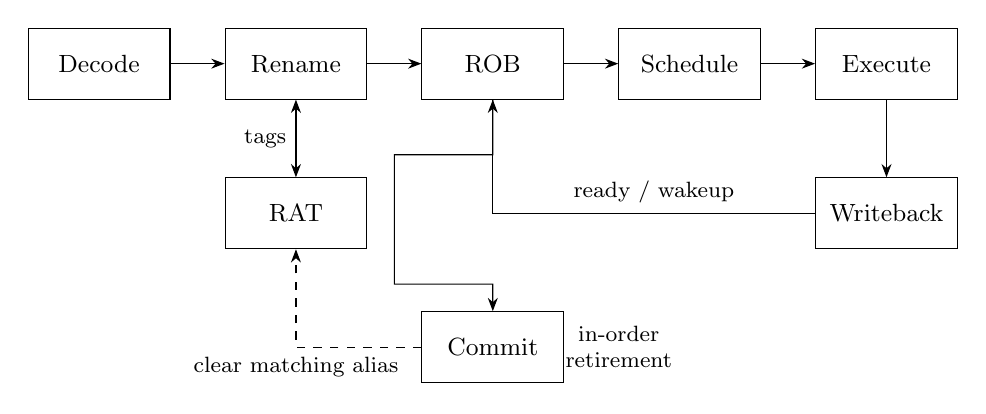
\begin{tikzpicture}[>=Stealth,font=\small,block/.style={draw,minimum width=1.8cm,minimum height=.9cm,align=center}]
\node[block] (decode) at (0,0) {Decode};
\node[block] (rename) at (2.5,0) {Rename};
\node[block] (rob) at (5,0) {ROB};
\node[block] (schedule) at (7.5,0) {Schedule};
\node[block] (execute) at (10,0) {Execute};
\draw[->] (decode)--(rename); \draw[->] (rename)--(rob);
\draw[->] (rob)--(schedule); \draw[->] (schedule)--(execute);
\node[block] (rat) at (2.5,-1.9) {RAT};
\node[block] (commit) at (5,-3.6) {Commit};
\node[block] (wb) at (10,-1.9) {Writeback};
\draw[<->] (rat.north)--node[left,font=\footnotesize]{tags}(rename.south);
\draw[->] (execute.south)--(wb.north);
\draw[->] (wb.west)-|node[pos=.25,above,font=\footnotesize]{ready / wakeup}(rob.south);
\draw[->] (rob.south)--++(0,-.7)--++(-1.25,0)--(3.75,-2.8)-|(commit.north);
\node[font=\footnotesize,align=center] at (6.6,-3.6) {in-order\\retirement};
\draw[->,dashed] (commit.west)-|node[pos=.5,below,font=\footnotesize]{clear matching alias}(rat.south);
\end{tikzpicture}

\caption{Renaming and scheduling dataflow. The ROB supplies instructions to scheduling, receives completion tags, and retires instructions in order.}\label{fig:architecture}
\end{figure}

\section{Results}
We compared widths one and two, load latencies of one and four cycles, and both scheduling policies. Table~\ref{tab:ooo} shows the two-wide CPI results. L1 and L4 refer to load latency in cycles.

\begin{table}[H]\centering\small
\begin{tabular}{lrrrr}
\toprule
Workload & IO / L1 & OOO / L1 & IO / L4 & OOO / L4 \\
\midrule
bzip2 & 0.503 & 0.500 & 0.511 & 0.501 \\
gcc & 0.504 & 0.500 & 0.518 & 0.500 \\
libq & 0.500 & 0.500 & 0.500 & 0.500 \\
mcf & 0.712 & 0.500 & 1.053 & 0.605 \\
\bottomrule\end{tabular}\caption{Two-wide CPI with in-order (IO) and out-of-order (OOO) scheduling.}\label{tab:ooo}\end{table}

\begin{figure}[H]\centering
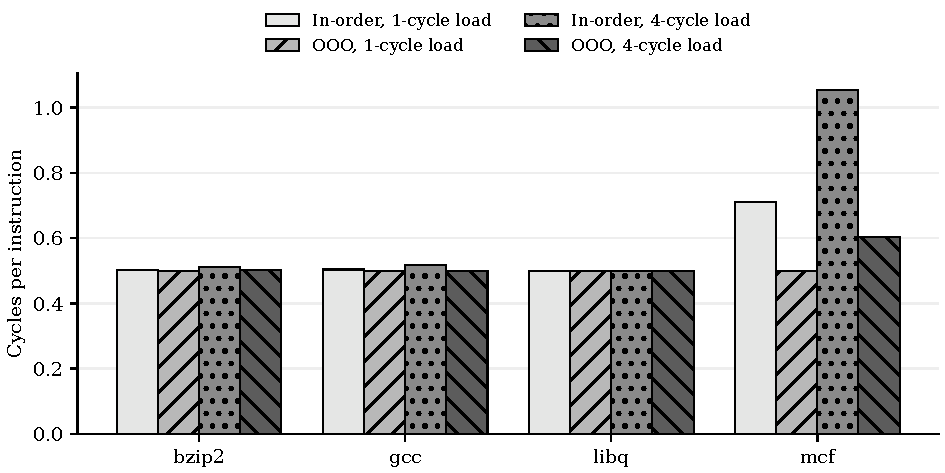
\includegraphics[width=\linewidth]{figures/scheduling_cpi.pdf}
\caption{Two-wide CPI by scheduling policy and load latency. Load latency and scheduling policy are varied independently.}\label{fig:results}
\end{figure}

The largest difference occurs on mcf. With four-cycle loads, out-of-order scheduling lowers CPI from 1.053 to 0.605, or about $1.74\times$ faster. Independent instructions can execute while an older load's dependents wait. The other streams change less: bzip2 improves from 0.511 to 0.501, gcc from 0.518 to 0.500, and libq stays at 0.500.

At width one, mcf improves from 1.451 to 1.001 CPI with four-cycle loads. Scheduling therefore helps even without a wider pipeline. Increasing width raises the possible issue rate; scheduling determines whether ready instructions are available to use it.




\end{document}
